\chapter{Methodology}
\label{sec:methodology}

This chapter explains what was and will be done within the duration of the whole project.

\section{Project Overview}
\label{sec:project_overview}

It has the main goal of creating a platform with all the games developed in the university's courses related to games. The games that will be available must have all their assets and required libraries in a single package that runs in Linux distributions without the need of installing any other package; they also must have a graphical installer for users without technical knowledge.

In order to achieve this goal, the games developed will be cataloged and cloned to a main GitHub organization (whenever possible). Two scripts will be created then, one to build games using SDL 1 and the other for SDL 2. The platform itself will be developed while all the other activities take place.

After that, a script will be generated to replicate the packaging system to all of the other games, making the necessary adjustments along the way. The games will be deployed to the website with all of their information and available installers.

The packaging scripts will be integrated and adapted to the platform, so that any student who posts a game will have the installers generated automatically.

\section{Task Division}
\label{sec:task_division}

This project is totally collaborative, it depends and relies on different classes and courses. Because of that, the work was divided among students and teachers, as illustrated in Figure \ref{fig:task_division}.

\begin{figure}[h!]
\centering
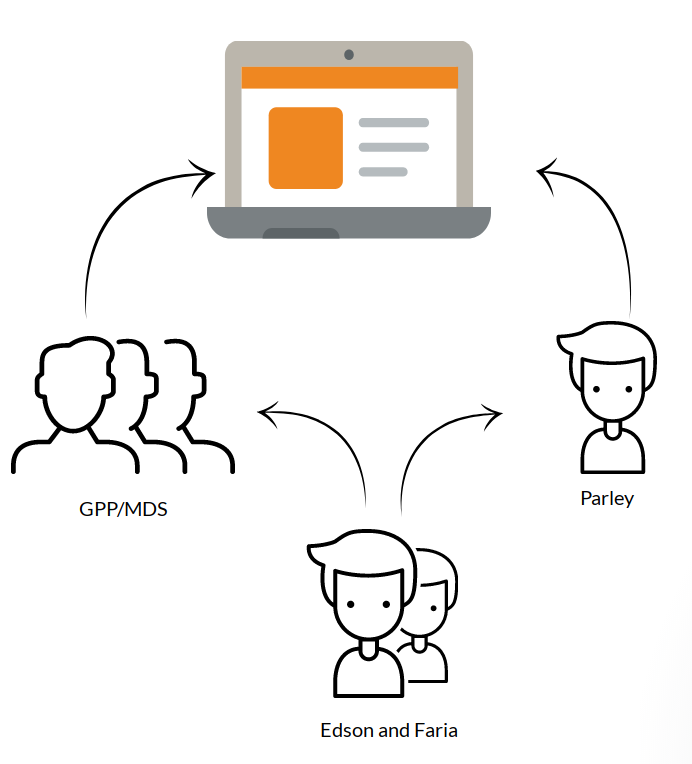
\includegraphics[width=200px,height=\textheight,keepaspectratio]{task_division}
\caption{Task Division}
\label{fig:task_division}
\end{figure}

Professor Edson and Mr. Faria were responsible for first cataloging the existing games. They will remain as helpers in the packaging system and main stakeholders for the team developing the website.

The team \textit{Plataforma de Jogos UnB} from the courses \textit{M\'etodos de Desenvolvimento de Software} (Software Development Methods) and \textit{Gest\~ao de Portfolios e Projetos} (Management of Portfolios and Projects) is in charge of creating the first version of the actual website with some of the features desired.

The scripts creation and their application on the games, their integration with the platform, as well as the evolution and maintenance of the platform after the courses are finished will be my responsibility.


\section{Game Gathering}
\label{sec:game_gathering}

The games selected for this first part of the project were the ones developed in this department, \textit{Faculdade UnB Gama} that is the Gama Campus of the University, since the course \textit{Introdu\c{c}\~ao aos Jogos Eletr\^onicos} (Introduction to Electronic Games) has been created here in the first semester of 2012. Because this work is being mostly held at FGA, and all the games developed here are compiled and run on Linux distributions, these were selected as first games for the platform. Another reason for this choice is the proximity with the students who created those games.

Professor Edson, that was ministering the course until last year, and Mr. Matheus Faria, the new teacher, first contacted the students and asked them to post their codes to GitHub. They cloned them into the \texttt{fgagamedev}\footnote{ \href{https://github.com/fgagamedev}{https://github.com/fgagamedev/} } GitHub organization.

After that, I was responsible for checking the status of the games, gathering information such as which of them compiled, which SDL version they used, which ones had licenses. Table \ref{tab:first_games} shows these initial results.

% \begin{center}
% \begin{longtable}{lcccc}
% \caption{Initial status of the selected games}
% \label{tab:first_games}

% % \rowcolors{2}{gray!30}{white}
% % \toprule
% \textbf{Name} & \textbf{Source?} & \textbf{License?} & \textbf{SDL} & \textbf{Compiles?} \\
% % \midrule
% Deadly Wish & y & n & 2 & n \\
% Strife of Mythology & y & n & 2 & y \\
% Travelling Will & y & n & 2 & y \\
% 7 Keys & y & MIT & 2 & n \\
% Babel & y & GPL 2 & 2 & y \\
% Terracota & y & MIT & 2 & n \\
% Dauphine & y & n & 2 & n \\
% Imagina na Copa & y & n & 2 & y \\
% Kays Against the World & y & n & 2 & y \\
% Ankhnowledge & y & GPL 2 & 1 & y \\
% The Last World War & n & - & - & - \\
% Post War & y & n & 1 & y \\
% War of the nets & y & GPL 2 & 2 & y \\
% Jack the Janitor & y & GPL 3 & 1 & y \\
% Drawing Attack & n & - & - & - \\
% Earth Attacks & n & - & - & - \\
% Emperor vs Aliens & y & n & 1 & y \\
% Ninja Siege & y & GPL 2 & 1 & y \\
% Space monkeys & y & GPL 2 & 1 & n \\
% Tacape & n & - & - & - \\
% % \bottomrule
% \end{longtable}
% \end{center}

\begin{table}[h!]
\centering
\caption{Initial status of the selected games}
\label{tab:first_games}
\rowcolors{2}{gray!30}{white}
\begin{tabular}{lcccc}
\toprule
\textbf{Name} & \textbf{Source?} & \textbf{License?} & \textbf{SDL} & \textbf{Compiles?} \\
\midrule
Deadly Wish & y & n & 2 & n \\
Strife of Mythology & y & n & 2 & y \\
Travelling Will & y & n & 2 & y \\
7 Keys & y & MIT & 2 & n \\
Babel & y & GPL 2 & 2 & y \\
Terracota & y & MIT & 2 & n \\
Dauphine & y & n & 2 & n \\
Imagina na Copa & y & n & 2 & y \\
Kays Against the World & y & n & 2 & y \\
Ankhnowledge & y & GPL 2 & 1 & y \\
The Last World War & n & - & - & - \\
Post War & y & n & 1 & y \\
War of the nets & y & GPL 2 & 2 & y \\
Jack the Janitor & y & GPL 3 & 1 & y \\
Drawing Attack & n & - & - & - \\
Earth Attacks & n & - & - & - \\
Emperor vs Aliens & y & n & 1 & y \\
Ninja Siege & y & GPL 2 & 1 & y \\
Space monkeys & y & GPL 2 & 1 & n \\
Tacape & n & - & - & - \\
\bottomrule
\end{tabular}
\end{table}

Out of 20 games created in \textit{Introdu\c{c}\~ao aos Jogos Eletr\^onicos}, 4 didn't have a known repository and 8 didn't have a license that allowed us to change them at that time. Mr. Faria and I were responsible for finding unknown games and getting the missing licenses. As result of this task, \textit{The Last World War} was added and 5 other had licenses acquired as shown in Table \ref{tab:final_games}.

\begin{table}[h!]
\centering
\caption{Game status after contacting developers}
\label{tab:final_games}
\rowcolors{2}{gray!30}{white}
\begin{tabular}{lccc}
\toprule
\textbf{} & \multicolumn{1}{l}{\textbf{License}} & \multicolumn{1}{l}{\textbf{SDL}} & \multicolumn{1}{l}{\textbf{Compiles}} \\
\midrule
Deadly Wish & GPL 3 & 2 & n \\
Strife of Mythology & GPL 2 & 2 & y \\
Travelling Will & MIT & 2 & y \\
7 Keys & MIT & 2 & n \\
Babel & GPL 2 & 2 & y \\
Terracota & MIT & 2 & n \\
Dauphine & MIT & 2 & n \\
Imagina na Copa & MIT & 2 & y \\
Kays Against the World & n & 2 & y \\
Ankhnowledge & GPL 2 & 1 & y \\
The Last World War & n & 1 & y \\
Post War & MIT & 1 & y \\
War of the nets & GPL 2 & 2 & y \\
Jack the Janitor & GPL 3 & 1 & y \\
Emperor vs Aliens & n & 1 & y \\
Ninja Siege & GPL 2 & 1 & y \\
Space monkeys & GPL 2 & 1 & n \\
\bottomrule
\end{tabular}
\end{table}


\section{Packaging}
\label{sec:packaging}

To create the installers for the games, professor Edson decided to use a folder structure that would be easy to understand to anyone familiar with Linux. Apart from the original directories in the repository, he added the folders \texttt{bin}, \texttt{dist}, \texttt{lib} and \texttt{linux}.

\begin{itemize}
\item \texttt{linux} would contain the scripts needed during compilation and also helpers to run the game after its building. When other OSs are added, there will be folders with the specifics for each one of them;
\item \texttt{lib} initially consists of the source of the libraries used by the games. They are built inside this folder as well, according to the Operating System the package is being built for;
\item \texttt{dist} includes the final installers, according to each supported OS. These can be distributed and installed in any supported computer;
\item \texttt{bin} has the compiled libraries and the game executable.

\end{itemize}

I added the directory \texttt{Qt} to use the Qt Installer Framework without having to install it system-wide. Figure \ref{fig:folder_structure} shows the folders and their contents to a SDL 1 project.

\begin{figure}[h!]
\centering
% 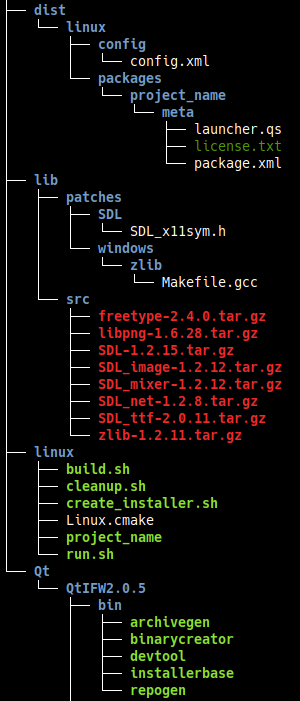
\includegraphics[width=150px,height=350px]{folder_structure}s
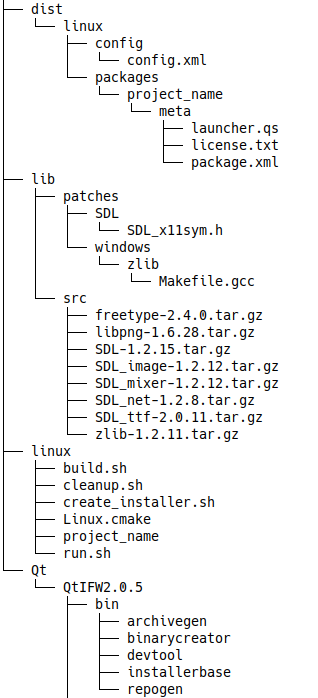
\includegraphics[width=150px,height=350px]{folder_structure2}
\caption{Folder tree}
\label{fig:folder_structure}
\end{figure}

\section{Platform Development}
\label{sec:platform}

The first version of the platform was developed using mixed development methods. During the first half of the semester, the Rational Unified Process was used. For the next part, Scrum and XP were chosen. This choice of development framework is because of how the courses are divided.

Throughout the RUP part of the development, the team created several documents to aid the development cycle, such as, vision, architecture document, class diagram, use case diagram, use case specification, test case specification.

These documents helped the team to understand the system requirements and how they should be implemented. The most experienced members also helped the others to learn the technologies to develop the website.


\section{Tools}
\label{sec:tools}

CMake is the chosen framework for generating the packages. It's suppose to help developers creating applications that run in several platforms, like Linux, Mac and Windows. It offers a lot options for that, like cross compilation and compilation directed to each of them. It is distributed under OSI-approved BSD 3-clause License and the minimum required version is 2.8.

For the graphical installer, Qt Installer Framework has been selected. It is easy to use and offers a nice GUI with all the necessary steps for installing a package, like license agreement and path choice. This framework is distributed under LGPLv3 license and the version being used is 2.0.5.

For the website development, Django was picked because of the previous knowledge the group had with it. To make the front end of the application, Facebook's React was chosen for the flexibility it gives to the user interface. They are both very scalable, have a big support on the community and are released under the BSD 3-clause license. The versions being used are the last ones at the beginning of the project, namely, 1.11.1, for Django, and 15.5.4, for React.

Python is the language for the packaging script because it must integrate with the Django webapp and its powerful easy to use API. It will also be the language for any other needed scripts. The least required version is 3.4, and it's licensed under an OSI-approved open source license.

To develop the scripts, a virtual machine running Debian Jessie was used. The VM was powered by Vagrant, version 1.9, that allows easy environment virtualization. It also enables a developer to test in several Operating Systems, which is required for the nature of this project. The computer hosting the script and used to its development has an Intel Core i5-6200U 2.3 GHz processor. It also has 8 GB of RAM and an NVIDIA GeForce 940M graphic processor.
